% SA-HEACS: Server-Assisted Hybrid Execution and AI-Optimized Cloud Shielding.
% Build:  python build.py           (or: latexmk -lualatex main.tex)
% Sections in sections/*.tex; TikZ figures in figures/*.tex; bibliography references.bib.
% Code listings and their outputs are read from code/ and code/outputs/ (run code/run_all.py
% first), so the paper always shows the shipped code and what it actually printed.
\documentclass[11pt,a4paper]{article}

% ---- Fonts and language (LuaLaTeX)
\usepackage{fontspec}
\usepackage{unicode-math}
\setmainfont{Libertinus Serif}
\setsansfont{Libertinus Sans}
\setmathfont{Libertinus Math}
\setmonofont[Scale=MatchLowercase,BoldFont=Inconsolatazi4-Bold.otf]{Inconsolatazi4-Regular.otf}
\usepackage[british]{babel}
\usepackage{csquotes}

% ---- Page layout
\usepackage[margin=25mm,headheight=14pt]{geometry}
\usepackage{setspace}
\setstretch{1.08}
\usepackage{microtype}
\usepackage{fancyhdr}
\pagestyle{fancy}
\fancyhf{}
\fancyhead[L]{\small\textsc{sa-heacs}}
\fancyhead[R]{\small Server-assisted execution against automated reverse engineering}
\fancyfoot[C]{\small\thepage}
\renewcommand{\headrulewidth}{0.4pt}
\fancypagestyle{plain}{\fancyhf{}\fancyfoot[C]{\small\thepage}\renewcommand{\headrulewidth}{0pt}}

% ---- Maths, tables, figures, lists
\usepackage{amsmath}
\usepackage{booktabs}
\usepackage{tabularx}
\usepackage{array}
\newcolumntype{Y}{>{\raggedright\arraybackslash}X}
\usepackage{graphicx}
\usepackage[font=small,labelfont=bf,margin=0pt]{caption}
\usepackage{enumitem}
\setlist{itemsep=2pt,topsep=4pt}
\usepackage[section]{placeins}

% ---- Colours, diagrams and plots
\usepackage{xcolor}
\definecolor{linkblue}{HTML}{1C5CAB}
\definecolor{accent}{HTML}{2F6FDB}
\definecolor{accentfill}{HTML}{E6EEFB}
\definecolor{promote}{HTML}{E59A1A}
\definecolor{boxgray}{HTML}{9A9890}
\definecolor{textgray}{HTML}{5F5E5A}
\definecolor{codebg}{HTML}{F7F6F3}
\usepackage{tikz}
\usetikzlibrary{positioning,fit,arrows.meta,calc,backgrounds}
\usepackage{pgfplots}
\pgfplotsset{compat=1.18}
\usepackage{pgfplotstable}
\usepgfplotslibrary{units}

% ---- Algorithms
\usepackage{algorithm}
\usepackage[noend]{algpseudocode}
\algrenewcommand\algorithmicrequire{\textbf{Input:}}
\algnewcommand{\LineComment}[1]{\Statex \hfill\textcolor{textgray}{\(\triangleright\) #1}}
\algrenewcommand{\algorithmiccomment}[1]{\hfill\textcolor{textgray}{\(\triangleright\) #1}}
\newcommand{\Kw}[1]{\textsc{#1}}

% ---- Code listings
\usepackage{listings}
\lstdefinestyle{py}{
  language=Python, basicstyle=\ttfamily\footnotesize, columns=fullflexible,
  keepspaces=true, backgroundcolor=\color{codebg}, frame=none,
  xleftmargin=4pt, xrightmargin=4pt, framesep=4pt, aboveskip=6pt, belowskip=6pt,
  keywordstyle=\color{accent!80!black}\bfseries, commentstyle=\color{textgray}\itshape,
  stringstyle=\color{promote!70!black}, showstringspaces=false,
  breaklines=true, breakatwhitespace=true,
  postbreak=\mbox{\textcolor{textgray}{$\hookrightarrow$}\space},
  numbers=left, numberstyle=\tiny\color{textgray}, numbersep=6pt}
\lstdefinestyle{out}{
  basicstyle=\ttfamily\footnotesize, columns=fullflexible, keepspaces=true,
  backgroundcolor=\color{codebg}, frame=leftline, rulecolor=\color{accent},
  xleftmargin=4pt, framesep=6pt, aboveskip=4pt, belowskip=8pt, breaklines=true}
\newcommand{\code}[1]{\texttt{#1}}
\newcommand{\tier}[1]{\texttt{#1}}

% ---- Bibliography: numeric, IEEE style, Biber
\usepackage[style=ieee,backend=biber,sorting=none,maxbibnames=8,minbibnames=3,
            dashed=false,urldate=iso,seconds=true]{biblatex}
\addbibresource{references.bib}

% ---- Links (last)
\usepackage[colorlinks=true,linkcolor=linkblue,citecolor=linkblue,urlcolor=linkblue,
            pdftitle={SA-HEACS: Server-Assisted Hybrid Execution and AI-Optimized Cloud
            Shielding Against Automated Reverse Engineering},pdfauthor={Kai Yi Ji}]{hyperref}
\usepackage{xurl}
\usepackage[capitalise,noabbrev]{cleveref}
\crefname{algorithm}{Algorithm}{Algorithms}
\crefname{lstlisting}{Listing}{Listings}

\title{\textbf{SA-HEACS: Server-Assisted Hybrid Execution and\\
       AI-Optimized Cloud Shielding Against\\ Automated Reverse Engineering}}
\author{Kai Yi Ji}
\date{Preprint, 16 October 2026}

\begin{document}
\maketitle
\thispagestyle{plain}

\begin{abstract}
\noindent
Automated, AI-assisted reverse-engineering pipelines now chain decompilers such as Ghidra,
dynamic instrumentation such as Frida, and large language models to recover program
semantics far faster than a human analyst. Classical client-side defences (obfuscation,
anti-debugging, tamper-proofing) raise the cost of analysis but cannot prevent recovery in
general, a limit made precise by the impossibility of virtual black-box obfuscation.
Client/server code splitting avoids that limit by not shipping the protected code.

This paper revisits client/server code splitting for AI-assisted reverse engineering. A
thin client shell holds no high-value intellectual property (IP) and reaches the product's
most valuable logic, kept on servers the vendor controls, through attested remote calls; we
call this design Server-Assisted Hybrid Execution and AI-Optimized Cloud Shielding
(SA-HEACS). The split and the attested call path follow prior work. We contribute two
mechanisms that make the split workable over a product's life: a learned orchestrator that
decides execution locality, micro-batches requests and prefetches likely work to offset the
latency and cost of remote execution; and a Dynamic Feature Promotion/Demotion Pipeline
that moves each feature between cloud-only, hybrid and client-local tiers as its IP value
and clone risk change.

We give a threat model, pseudocode and runnable Python for the attested call path, the
orchestrator and the lifecycle policy, and a discrete-event simulation of cost and latency.
In that simulation, a 5\,ms batching window cuts accelerator time per request about eightfold
for 6\,ms of extra 95th-percentile latency, and prefetching the two most likely next
operations hides the network round trip for 68\% of steps at the price of 132\% extra
compute. Keeping the code on the server removes it from the attacker's machine, which defeats
static decompilation and memory dumping of that code. It does not stop black-box extraction
of functionality through the API: query-based model extraction, output-based cloning and
account abuse remain, and we treat them as residual risks with rate-limiting, watermarking
and anomaly-detection mitigations rather than claiming them solved.
\end{abstract}

\vspace{2pt}
\noindent\textbf{Keywords:} software protection; reverse engineering; client/server code
splitting; obfuscation; remote attestation; computation offloading; model extraction; ML
serving.

\section{Introduction}\label{sec:intro}

Code that runs on hardware the attacker controls can eventually be read, so the strongest
protection for an algorithm is not to ship it. Software protection has long accepted that
every client-side defence is a cost multiplier, not a barrier
\cite{collberg1997taxonomy,collberg2002watermarking,schrittwieser2016obfuscation}. Studies of
professional attackers show that they defeat layered obfuscation by combining static and
dynamic analysis and by focusing on the small region that holds the asset
\cite{ceccato2017hackers}.

Two shifts make that cost multiplier smaller. First, analysis tools are scriptable end to
end: Ghidra exposes a headless analyser and scripting API \cite{nsa2019ghidra}, frameworks
such as angr automate symbolic and dynamic analysis \cite{shoshitaishvili2016sok}, and Frida
injects JavaScript hooks into running processes to trace, patch and dump memory
\cite{frida}. Second, learned models now lift binaries toward readable source and recover
names and types: DIRE and DIRTY predict identifier names and types from decompiler output
\cite{lacomis2019dire,chen2022dirty}, and LLM4Decompile trains language models to decompile
x86 binaries end to end \cite{tan2024llm4decompile}. An automated reverse-engineering agent
(the original SA-HEACS blueprint calls such a toolkit an \enquote{REA}) can therefore chain
dumping, decompilation and semantic recovery with little human effort. The scarce resource
for the attacker is no longer analyst time; it is access to the code.

SA-HEACS removes that access for the code that matters. It splits an application into a
thin client shell, which handles input, local rendering and commodity features, and a set
of server-side services that hold the high-value IP. The idea of hiding a program slice on
a trusted server is old \cite{zhang2003hiding}, as is offloading work from a constrained
client \cite{cuervo2010maui,chun2011clonecloud,kang2017neurosurgeon}. What is new here is the
combination of three things: an explicit IP-centric partitioning rule; a learned
orchestrator that makes the economics of remote execution workable through locality
routing, micro-batching and prefetch; and a lifecycle policy that moves features between
tiers as their value decays.

This paper makes five contributions:
\begin{enumerate}
  \item An architecture that separates a zero-IP client shell from attested, segmented
        server clusters, with a request protocol (\cref{sec:arch}).
  \item A threat model that states which reverse-engineering attacks the design removes and
        which it does not (\cref{sec:threat,sec:security}).
  \item An orchestrator design with pseudocode and runnable Python for locality routing,
        micro-batching and Markov prefetch (\cref{sec:orch}).
  \item A Dynamic Feature Promotion/Demotion Pipeline that scores each feature's IP value
        and clone risk and moves it between cloud-only and client-local execution
        (\cref{sec:lifecycle}).
  \item An evaluation methodology and a reproducible simulation of cost and latency
        trade-offs, with the limits of what simulation can show (\cref{sec:eval}).
\end{enumerate}
All code is listed in \cref{app:code} and runs as shipped; every program output quoted in
the text is read from the output of that code.

\section{Background and related work}\label{sec:related}

Prior work establishes that client-side protection only delays analysis, that server-side
execution has been used for performance more than for secrecy, and that a remote API leaks
its function through its outputs. SA-HEACS sits where those three lines meet.

\subsection{Obfuscation and its limits}
Collberg, Thomborson and Low catalogued obfuscating transformations by potency, resilience
and cost \cite{collberg1997taxonomy}, and later framed obfuscation, watermarking and
tamper-proofing as complementary tools \cite{collberg2002watermarking,collberg2009surreptitious}.
Barak et al.\ proved that virtual black-box obfuscation is impossible for general programs:
some functions leak properties through any obfuscated form \cite{barak2012impossibility}.
Indistinguishability obfuscation is constructible in theory \cite{garg2013candidate} but
remains far too slow for production code. Empirically, Schrittwieser et al.\ found that most
practical obfuscations fall to modern static and dynamic analysis given enough effort
\cite{schrittwieser2016obfuscation}, and Banescu et al.\ showed that symbolic execution
defeats many transformations unless they are designed against it \cite{banescu2016symbolic}.
Ceccato et al.\ observed professional penetration testers and found that they locate and
attack the protected asset rather than deobfuscating the whole program
\cite{ceccato2017hackers}.

\subsection{Automated and learning-based reverse engineering}
Scriptable platforms turn reverse engineering into a pipeline. Ghidra provides headless
batch analysis and a scripting API \cite{nsa2019ghidra}; angr packages the offensive
binary-analysis techniques surveyed by Shoshitaishvili et al.\ \cite{shoshitaishvili2016sok};
Frida injects instrumentation into live processes on desktop and mobile platforms
\cite{frida}. Learned models then improve the output: DIRE and DIRTY predict variable names
and types for decompiled code \cite{lacomis2019dire,chen2022dirty}, and LLM4Decompile reports
end-to-end decompilation of compiled binaries by fine-tuned language models
\cite{tan2024llm4decompile}. These tools lower the human effort per target, which weakens
defences whose value rested on analyst time.

\subsection{Program splitting and computation offloading}
Zhang and Gupta proposed hiding critical program slices on a trusted server so that the
client binary is incomplete \cite{zhang2003hiding}; SA-HEACS generalises this from slices
to whole features with a managed lifecycle. Offloading systems such as MAUI
\cite{cuervo2010maui}, CloneCloud \cite{chun2011clonecloud} and Neurosurgeon
\cite{kang2017neurosurgeon} partition work between device and cloud to save energy or
latency, and cloud gaming systems stream rendered output to thin clients
\cite{huang2013gaminganywhere}. These systems optimise performance; secrecy of the offloaded
code is not their goal, so they freely move code to the client when that is faster.
SA-HEACS reverses the priority: the security tier is a hard constraint and performance is
optimised inside it.

\subsection{Attestation}
Remote attestation lets a server judge the state of a client before serving it. RFC~9334
defines the roles of attester, verifier and relying party \cite{rfc9334}. Mobile platforms
provide attestation services, Google Play Integrity \cite{google_playintegrity} and Apple
App Attest \cite{apple_appattest}, and trusted execution environments such as Intel SGX add
hardware-rooted quotes \cite{costan2016sgx}. Attestation raises the cost of driving the API
from a modified client, but it does not keep a legitimate client from observing its own
inputs and outputs.

\subsection{Model extraction through APIs}
Keeping code on a server does not keep its function secret. Tramèr et al.\ extracted models
from commercial prediction APIs through queries alone \cite{tramer2016stealing}; Orekondy et
al.\ trained functionally similar \enquote{knockoff} networks from black-box outputs
\cite{orekondy2019knockoff}; Jagielski et al.\ studied high-fidelity extraction
\cite{jagielski2020extraction}. Defences include query-distribution monitoring such as
PRADA \cite{juuti2019prada} and watermarks embedded in a model's behaviour
\cite{adi2018watermarking}. These results bound what SA-HEACS can claim (\cref{sec:security}).

\subsection{Serving systems and batching}
The orchestrator draws on ML serving work. Clipper introduced adaptive batching for
latency-bounded prediction serving \cite{crankshaw2017clipper}; Orca added iteration-level
scheduling for transformer inference \cite{yu2022orca}; vLLM's PagedAttention raised batch
capacity by managing key--value cache memory \cite{kwon2023vllm}. Resource Central predicts
virtual-machine behaviour to inform allocation \cite{cortez2017resourcecentral}, and
predictive prefetching has long been used to hide web latency
\cite{padmanabhan1996prefetching}. Dean and Barroso describe why tail latency, not the mean,
governs user experience at scale \cite{dean2013tail}.

\section{Threat model}\label{sec:threat}

The attacker fully controls the client device and holds a valid account, but cannot read
server memory or storage. This is the standard man-at-the-end setting
\cite{collberg2009surreptitious} with a trusted server added.

\paragraph{Assets.} (A1) Proprietary algorithms and model weights in cloud-only features.
(A2) Server-side state such as cached intermediate results. (A3) The service's availability
and cost envelope. (A4) Lower-value code shipped in the client shell, which is explicitly
not protected beyond standard obfuscation.

\paragraph{Attacker capabilities.} The attacker can decompile and patch the client binary,
hook any function with dynamic instrumentation, read and modify process memory, intercept
traffic after TLS termination on their own device, and script all of this with an AI agent
that plans, runs tools and summarises findings. They can create many accounts, subject to
the vendor's sign-up controls, and send any sequence of valid queries.

\paragraph{Trust assumptions.} The server fleet, its hypervisor and the build pipeline are
trusted; insiders and cloud-provider compromise are out of scope. Platform attestation
services \cite{google_playintegrity,apple_appattest} are assumed sound, though we treat a
bypassed attestation as a degraded mode rather than a total failure. Side channels on shared
server hardware are out of scope but discussed in \cref{sec:discussion}.

\paragraph{Attacker goals.} \Cref{tab:goals} lists the goals we consider and whether the
design addresses them.

\begin{table}[htbp]
\centering
\caption{Attacker goals and their status under SA-HEACS.}\label{tab:goals}
\small
\begin{tabularx}{\linewidth}{@{}l Y l@{}}
\toprule
Goal & Example & In scope \\
\midrule
G1 Code recovery      & Recover source or weights of a cloud-only feature & Yes \\
G2 Functional cloning & Train or build a substitute from input--output pairs & Yes, as residual risk \\
G3 Free-riding        & Use a cloned or patched client to call the API without paying & Yes \\
G4 Shell cloning      & Copy the client UI and commodity features & Accepted \\
G5 Denial of service  & Exhaust GPU capacity with costly requests & Partly \\
G6 Server compromise  & Exploit the RPC surface to read server memory & Out of scope; standard hardening \\
\bottomrule
\end{tabularx}
\end{table}

\section{SA-HEACS architecture}\label{sec:arch}

SA-HEACS has three components joined by one attested request path: the client shell, the
orchestrator and the secure clusters (\cref{fig:arch}).

\begin{figure}[htbp]
\centering
% Figure 1: SA-HEACS architecture. Everything in the dashed client box is attacker-readable.
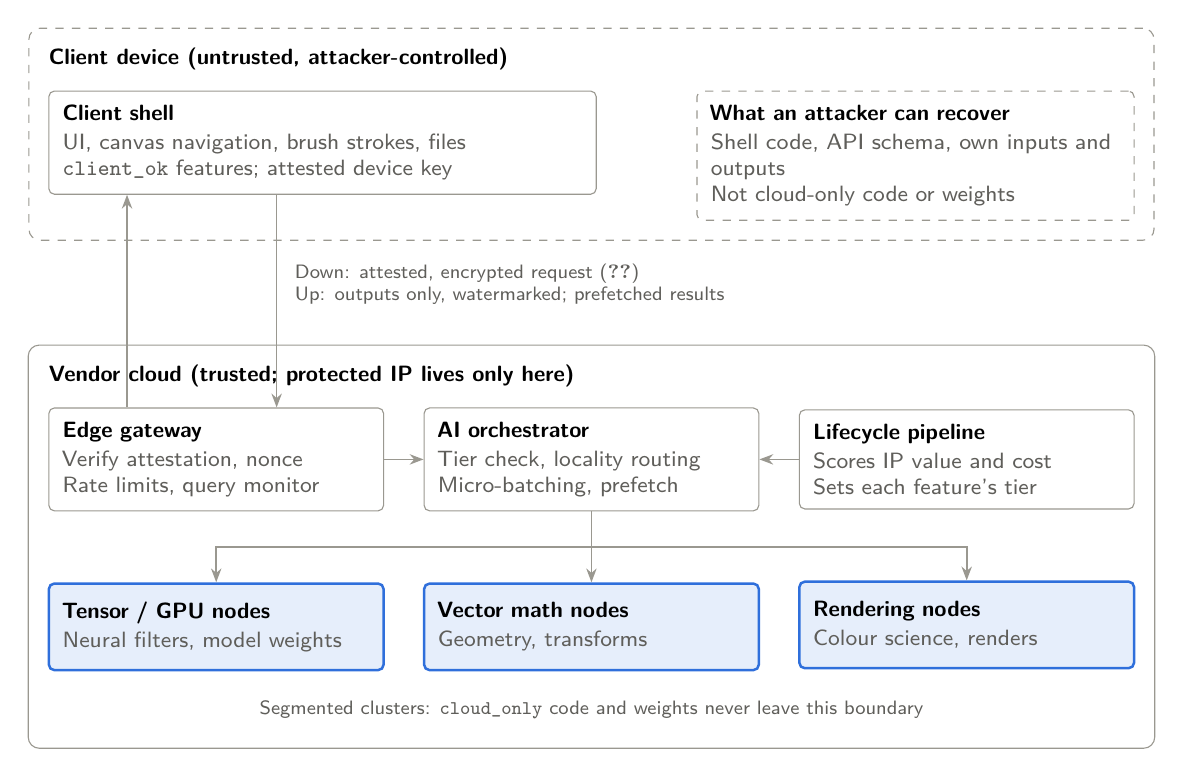
\begin{tikzpicture}[
    font=\sffamily\footnotesize,
    box/.style={draw=boxgray, rounded corners=2pt, fill=white, align=left,
                inner sep=5pt, text width=#1},
    box/.default=3.9cm,
    core/.style={box=3.9cm, draw=accent, line width=0.9pt, fill=accentfill, minimum height=11mm},
    region/.style={rounded corners=4pt, inner sep=7pt},
    title/.style={font=\sffamily\footnotesize\bfseries, anchor=south west, inner sep=0pt},
    arr/.style={-{Stealth[length=5pt]}, draw=boxgray, line width=0.6pt},
    lbl/.style={font=\sffamily\scriptsize, text=textgray, align=left}]

  % cloud side (laid out first; the client row is placed above it)
  \node[box] (edge) {\textbf{Edge gateway}\\[1pt]
      \textcolor{textgray}{Verify attestation, nonce}\\\textcolor{textgray}{Rate limits, query monitor}};
  \node[box, right=5mm of edge] (orch) {\textbf{AI orchestrator}\\[1pt]
      \textcolor{textgray}{Tier check, locality routing}\\\textcolor{textgray}{Micro-batching, prefetch}};
  \node[box, right=5mm of orch] (life) {\textbf{Lifecycle pipeline}\\[1pt]
      \textcolor{textgray}{Scores IP value and cost}\\\textcolor{textgray}{Sets each feature's tier}};
  \node[core, below=9mm of edge] (gpu) {\textbf{Tensor / GPU nodes}\\[1pt]\textcolor{textgray}{Neural filters, model weights}};
  \node[core, below=9mm of orch] (vec) {\textbf{Vector math nodes}\\[1pt]\textcolor{textgray}{Geometry, transforms}};
  \node[core, below=9mm of life] (ren) {\textbf{Rendering nodes}\\[1pt]\textcolor{textgray}{Colour science, renders}};
  \node[lbl, below=2.5mm of vec, align=center] (seg) {Segmented clusters: \tier{cloud\_only} code and weights never leave this boundary};
  \node[title] (stitle) at ($(edge.north west)+(0,2.5mm)$) {Vendor cloud (trusted; protected IP lives only here)};
  \begin{scope}[on background layer]
    \node[region, draw=boxgray, fit=(edge)(life)(gpu)(ren)(seg)(stitle)] (cloud) {};
  \end{scope}

  % client side
  \node[box=6.6cm, above=27mm of edge.north west, anchor=south west] (shell) {\textbf{Client shell}\\[1pt]
      \textcolor{textgray}{UI, canvas navigation, brush strokes, files}\\
      \textcolor{textgray}{\tier{client\_ok} features; attested device key}};
  \node[box=5.2cm, dashed, anchor=north east] (recover) at (life.north east |- shell.north)
      {\textbf{What an attacker can recover}\\[1pt]
      \textcolor{textgray}{Shell code, API schema, own inputs and outputs}\\
      \textcolor{textgray}{Not cloud-only code or weights}};
  \node[title] (ctitle) at ($(shell.north west)+(0,2.5mm)$) {Client device (untrusted, attacker-controlled)};
  \begin{scope}[on background layer]
    \node[region, draw=boxgray, dashed, fit=(shell)(recover)(ctitle)] (client) {};
  \end{scope}

  % request path: vertical arrows between the shell and the edge gateway
  \coordinate (dn) at ($(edge.north west)+(2.9,0)$);
  \coordinate (up) at ($(edge.north west)+(1.0,0)$);
  \draw[arr] (dn |- shell.south) -- node[lbl, right=3pt, pos=0.42]
      {Down: attested, encrypted request (\cref{alg:rpc})\\Up: outputs only, watermarked; prefetched results} (dn);
  \draw[arr] (up) -- (up |- shell.south);
  \draw[arr] (edge) -- (orch);
  \draw[arr] (life) -- (orch);
  \draw[arr] (orch.south) -- ++(0,-4.5mm) -| (gpu.north);
  \draw[arr] (orch.south) -- (vec.north);
  \draw[arr] (orch.south) -- ++(0,-4.5mm) -| (ren.north);
\end{tikzpicture}

\caption{SA-HEACS architecture: client shell, attested RPC, orchestrator and segmented
clusters. Everything inside the dashed client boundary is assumed readable by the attacker;
the blue clusters hold the protected IP and return only outputs.}
\label{fig:arch}
\end{figure}

\subsection{Client shell (the untrusted boundary)}
The shell handles input, canvas navigation, local brush strokes, file handling, UI
rendering and any feature in the \tier{client\_ok} tier. It holds no cloud-only code or
weights. Its only secrets are a device identity bound to platform attestation and
short-lived session keys. We assume it will be fully decompiled and cloned; the design goal
is that a perfect clone gains a UI and commodity features, not the protected capabilities.

\subsection{Secure clusters (the protected core)}
Cloud-only features run as segmented microservices grouped by hardware need: tensor and GPU
inference, vector and geometry maths, and rendering or colour-science pipelines. Each
feature runs under its own service identity with least-privilege access to its weights.
Clients never receive code, weights or intermediate tensors that would let a substitute be
rebuilt more cheaply than by black-box queries; responses carry only the final output at the
resolution the product needs.

\subsection{Orchestrator (the control plane)}
The orchestrator sits between the edge and the clusters. It enforces each feature's tier,
routes \tier{hybrid} and \tier{client\_ok} work to the cheaper side, groups compatible
requests into micro-batches, and prefetches likely next operations. \Cref{sec:orch} details
it.

\subsection{Request protocol}
Every remote call carries an attestation-bound signature, a fresh nonce and an encrypted
body (\cref{alg:rpc}). The client derives a per-request key from an ephemeral X25519
exchange \cite{bernstein2006curve25519,rfc7748} with the server's static key, expanded with
HKDF \cite{rfc5869} using the nonce as salt, and encrypts with AES-GCM \cite{nist80038d}.
The ephemeral public key, nonce and timestamp are signed with an Ed25519 device key
\cite{bernstein2012ed25519,rfc8032} that, in production, is bound to a platform attestation
verdict, and the same bytes are passed to AES-GCM as associated data. The server rejects
stale or replayed requests and unattested devices before any protected code runs. Request
and response use disjoint 12-byte GCM nonces under the per-request key.

\begin{algorithm}[htbp]
\caption{Attested invocation of a cloud-only feature}\label{alg:rpc}
\small
\begin{algorithmic}[1]
\Statex \textbf{Client:}
\State \((e, E) \gets \Kw{X25519.Generate}()\)
\State \(n \gets \Kw{Random}(16)\); \(t \gets \Kw{Now}()\)
\State \(\sigma \gets \Kw{Sign}(K_{\text{device}},\, E \parallel n \parallel t)\) \Comment{\(K_{\text{device}}\) bound to platform attestation}
\State \(k \gets \Kw{HKDF}(\Kw{ECDH}(e, S_{\text{pub}}),\ \text{salt}=n)\)
\State \(c \gets \Kw{AES-GCM.Enc}(k,\ n[0{:}12],\ \{\text{feature}, \text{args}\},\ \text{aad}=E \parallel n \parallel t)\)
\State \textbf{send} \((\text{device\_id}, E, n, t, \sigma, c)\)
\Statex \textbf{Server:}
\If{\(|\Kw{Now}() - t| > \Delta\) \textbf{or} \(n \in \text{SeenNonces}\)} \textbf{reject} \EndIf
\If{\textbf{not} \(\Kw{Verify}(\text{AttestedKey}[\text{device\_id}], \sigma)\)} \textbf{reject} \EndIf
\If{\textbf{not} \(\Kw{RateLimiter.Allow}(\text{account}, \text{feature})\)} \textbf{reject} \Comment{\cref{sec:security}} \EndIf
\State \(k \gets \Kw{HKDF}(\Kw{ECDH}(S_{\text{priv}}, E),\ \text{salt}=n)\)
\State \(\text{req} \gets \Kw{AES-GCM.Dec}(k,\ n[0{:}12],\ c,\ \text{aad})\)
\State \(y \gets \Kw{Orchestrator.Submit}(\text{req.feature}, \text{req.args})\) \Comment{\cref{sec:orch}}
\State \Return \(\Kw{AES-GCM.Enc}(k,\ n[12{:}16] \parallel 0^{8},\ \Kw{Watermark}(y),\ \text{aad})\)
\end{algorithmic}
\end{algorithm}

The runnable version, \code{attested\_rpc.py} (\cref{app:rpc}), implements lines 1--8 and
10--13, without the rate limiter and watermark, using the Python \code{cryptography} package
\cite{pyca_cryptography} and FastAPI \cite{fastapi}. Running it shows a valid call returning
the filtered result and a cloned client with an unattested key rejected with HTTP~401. In
production, line~8 would consume a Play Integrity or App Attest verdict
\cite{google_playintegrity,apple_appattest} instead of a locally registered Ed25519 key, and
the nonce cache would be bounded by the skew window \(\Delta\).

\section{The AI orchestrator}\label{sec:orch}

The orchestrator's job is to make remote execution cheap and fast enough that keeping IP
server-side is commercially viable. It does three things, and the security tier constrains
all of them: no optimisation may move a \tier{cloud\_only} feature to the client.

\subsection{Locality routing}
For \tier{hybrid} and \tier{client\_ok} features, a classifier trained on telemetry predicts
whether remote execution will finish sooner than local execution, from payload size,
estimated work, measured round-trip time, device capability and battery level. This follows
the partitioning logic of MAUI and Neurosurgeon \cite{cuervo2010maui,kang2017neurosurgeon},
with the tier check placed first (\cref{alg:route}).

\begin{algorithm}[htbp]
\caption{\Kw{Route}\((r)\)}\label{alg:route}
\small
\begin{algorithmic}[1]
\If{\(r.\text{tier} = \tier{cloud\_only}\)} \Return \Kw{Cloud} \Comment{hard security constraint} \EndIf
\If{\(r.\text{tier} = \tier{client\_ok}\) \textbf{and} \(r.\text{rtt} > \text{RTT}_{\max}\)} \Return \Kw{Local} \EndIf
\State \(p \gets \Kw{Model}.P(\text{remote faster} \mid \text{payload}, \text{work}, \text{rtt}, \text{device}, \text{battery})\)
\State \Return \Kw{Cloud} \textbf{if} \(p \ge 0.5\) \textbf{else} \Kw{Local}
\end{algorithmic}
\end{algorithm}

\code{orchestrator.py} (\cref{app:orch}) trains a scikit-learn
\code{GradientBoostingClassifier} \cite{pedregosa2011sklearn} on 3,000 synthetic telemetry
records and reaches 0.956 accuracy on 1,000 held-out records. The labels come from a simple
latency model, so this number shows that the pipeline works, not that a real router would be
this accurate.

\subsection{Micro-batching}
Accelerators amortise fixed per-call cost (kernel launch, weight reads) across a batch. The
orchestrator holds requests for the same feature for up to a window of \(W\) milliseconds
or until \(B\) requests arrive, then runs one batched call (\cref{alg:batch}), as Clipper
does for model serving \cite{crankshaw2017clipper}. Requests from different tenants share a
batch, but each row's output is returned only to its sender, and no state persists across
rows.

\begin{algorithm}[htbp]
\caption{\Kw{MicroBatcher.Submit}(feature \(f\), input \(x\))}\label{alg:batch}
\small
\begin{algorithmic}[1]
\State \(Q[f].\Kw{Append}((x, \text{future}))\)
\If{\(|Q[f]| \ge B\)} \Kw{Flush}\((f)\)
\ElsIf{no timer for \(f\)} start timer\((W, \Kw{Flush}(f))\)
\EndIf
\State \Return \textbf{await} future
\Statex \textbf{procedure} \Kw{Flush}\((f)\)
\State \(\text{items} \gets Q[f]\); \(Q[f] \gets [\,]\)
\State \(Y \gets \Kw{Kernel}_f(\Kw{Stack}(x \text{ for } x \in \text{items}))\) \Comment{one accelerator call}
\For{each \((\text{item}, y)\)} \(\text{item.future.Resolve}(y)\) \EndFor
\end{algorithmic}
\end{algorithm}

The \code{asyncio} implementation in \cref{app:orch} serves a burst of 200 requests in 4
batched calls (wall-clock time depends on the machine). \Cref{sec:eval} measures the cost
and latency trade-off of \(W\).

\subsection{Predictive prefetch}
A first-order Markov model over each user's feature sequence predicts the next operation
(\cref{alg:prefetch}). When the user invokes feature \(a\), the orchestrator speculatively
computes the top-\(k\) features \(b\) with \(P(b \mid a)\) above a threshold and pushes the
results to the client cache. A hit replaces a network round trip with a local read; a miss
wastes compute. With a toy session of ten steps, the model in \cref{app:orch} learns that
after \code{denoise} the user goes to \code{upscale} or \code{colorize}.

\begin{algorithm}[htbp]
\caption{\Kw{OnInvoke}(user \(u\), feature \(a\))}\label{alg:prefetch}
\small
\begin{algorithmic}[1]
\State \(M[u.\text{prev}][a] \mathrel{+}= 1\); \(u.\text{prev} \gets a\)
\For{\(b \in \Kw{TopK}(M[a])\) with \(M[a][b] / \sum M[a] \ge p_{\min}\)}
  \If{\(\Kw{Budget.Allow}(u, b)\)} schedule speculative \(\Kw{Run}(b, u.\text{state})\) at low priority \EndIf
\EndFor
\end{algorithmic}
\end{algorithm}

Prefetched results are outputs, not code, so prefetch does not weaken the zero-footprint
rule. It does increase the volume of outputs a client receives, which matters for
extraction risk (\cref{sec:security}).

\section{Dynamic feature promotion and demotion pipeline}\label{sec:lifecycle}

A feature's tier is a business decision that changes over time: new IP starts cloud-only,
and it moves toward the client only when its secrecy is worth less than the cost and latency
of serving it remotely. Moves toward the client are one-way in practice, because shipped
code must be assumed public, so the pipeline makes demotion (back to the cloud) automatic
and gates promotion to the client on a human reviewer.

\subsection{Tiers}
\begin{itemize}
  \item \textbf{\tier{cloud\_only} (incubation).} Code and weights exist only on servers.
        New or high-value features start here.
  \item \textbf{\tier{hybrid}.} The server stays authoritative, but an obfuscated or
        reduced-quality client fallback is allowed for offline use or poor networks.
  \item \textbf{\tier{client\_ok} (commoditised).} The feature ships in the client package,
        protected only by standard obfuscation \cite{collberg1997taxonomy}, and runs locally
        to save server cost and latency.
\end{itemize}

\begin{figure}[htbp]
\centering
% Figure 2: feature tier state machine with the Section 6.3 thresholds.
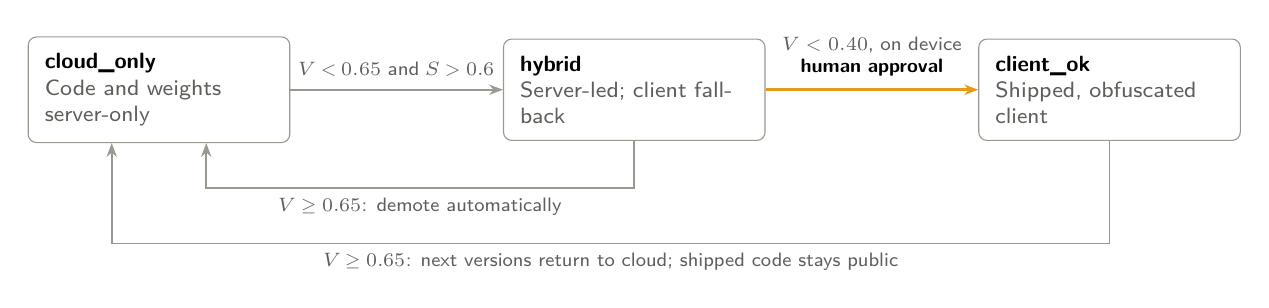
\begin{tikzpicture}[
    font=\sffamily\footnotesize,
    st/.style={draw=boxgray, rounded corners=3pt, fill=white, align=left, inner sep=6pt,
               text width=2.9cm, minimum height=12mm},
    arr/.style={-{Stealth[length=5pt]}, draw=boxgray, line width=0.6pt},
    lbl/.style={font=\sffamily\scriptsize, text=textgray, align=center}]
  \node[st] (c) {\textbf{cloud\_only}\\\textcolor{textgray}{Code and weights server-only}};
  \node[st, right=27mm of c] (h) {\textbf{hybrid}\\\textcolor{textgray}{Server-led; client fallback}};
  \node[st, right=27mm of h] (k) {\textbf{client\_ok}\\\textcolor{textgray}{Shipped, obfuscated client}};

  \draw[arr] (c) -- node[lbl, above=1pt, text width=2.5cm] {\(V < 0.65\) and \(S > 0.6\)} (h);
  \draw[arr, draw=promote, line width=1.1pt] (h) -- node[lbl, above=1pt, text width=2.6cm]
      {\(V < 0.40\), on device\\\textcolor{black}{\textbf{human approval}}} (k);
  \draw[arr] (h.south) -- ++(0,-6mm) -| node[lbl, below, pos=0.25] {\(V \ge 0.65\): demote automatically} ($(c.south)+(0.6,0)$);
  \draw[arr] (k.south) -- ++(0,-13mm) -| node[lbl, below, pos=0.25] {\(V \ge 0.65\): next versions return to cloud; shipped code stays public} ($(c.south)+(-0.6,0)$);
\end{tikzpicture}

\caption{Feature tier state machine with the thresholds of \cref{sec:transition}
(\(V\) = IP value, \(S\) = serving pressure; every promotion first waits out a 30-day dwell
time). Only the move to \tier{client\_ok} needs a person to approve it, because shipped code
cannot be recalled; every move back toward the cloud is automatic.}
\label{fig:lifecycle}
\end{figure}

\subsection{Scoring}
The pipeline computes two scores per feature from product and telemetry signals. IP value
\(V\) combines novelty \(N\), share of premium revenue \(R\), competitor parity \(C\) (how
closely public competitors match the output) and whether the method is published,
\(P \in \{0,1\}\):
\begin{equation}\label{eq:value}
  V = 0.35\,N + 0.35\,R + 0.20\,(1 - C) + 0.10\,(1 - P).
\end{equation}
Serving pressure \(S\) compares cost per 1,000 invocations \(c\) and 95th-percentile
latency \(\ell\) to budgets \(c_{\max}\) and \(\ell_{\max}\):
\begin{equation}\label{eq:pressure}
  S = \min\!\left(1,\ \tfrac{1}{2}\,\frac{c}{c_{\max}} + \tfrac{1}{2}\,\frac{\ell}{\ell_{\max}}\right).
\end{equation}
The weights are illustrative; an organisation would set them with its product and legal
teams. Clone risk enters through \(C\) and \(P\): once competitors reach parity or the
method is published, secrecy protects little.

\subsection{Transition policy}\label{sec:transition}
The policy uses a hysteresis band (\(V_{\text{hi}} = 0.65\), \(V_{\text{lo}} = 0.40\)) and
a minimum dwell time of 30 days so that noisy signals do not make a feature oscillate
between tiers (\cref{alg:decide}).

\begin{algorithm}[htbp]
\caption{\Kw{Decide}(feature \(f\), signals \(s\))}\label{alg:decide}
\small
\begin{algorithmic}[1]
\State \(V \gets \Kw{IPValue}(s)\); \(S \gets \Kw{ServingPressure}(s)\) \Comment{\cref{eq:value,eq:pressure}}
\If{\(V \ge V_{\text{hi}}\) \textbf{and} \(f.\text{tier} \ne \tier{cloud\_only}\)} \Return \tier{cloud\_only} \Comment{demote now; reversible} \EndIf
\If{\(f.\text{days\_in\_tier} < \text{MIN\_DWELL}\)} \Return \(f.\text{tier}\) \EndIf
\If{\(f.\text{tier} = \tier{cloud\_only}\) \textbf{and} \(V < V_{\text{hi}}\) \textbf{and} \(S > 0.6\)} \Return \tier{hybrid} \EndIf
\If{\(f.\text{tier} = \tier{hybrid}\) \textbf{and} \(V < V_{\text{lo}}\) \textbf{and} \(s.\text{on\_device\_feasible}\)}
  \State \Return \tier{client\_ok} pending \(\Kw{Approve}(f)\) \Comment{irreversible: human gate}
\EndIf
\State \Return \(f.\text{tier}\)
\end{algorithmic}
\end{algorithm}

\code{lifecycle.py} (\cref{app:lifecycle}) runs one simulated year for a feature whose
novelty and revenue share decay while competitor parity rises and the method is published on
day~201. The feature moves from \tier{cloud\_only} to \tier{hybrid} on day~97
(\(V = 0.648\), \(S = 0.908\)) and to \tier{client\_ok} on day~201 (\(V = 0.36\)), the day
publication removes its remaining secrecy value.

\subsection{Automated packaging}
A promotion to \tier{client\_ok} triggers a build step that compiles the feature for client
targets, applies the shell's standard obfuscation profile, and adds it to the next client
release behind a feature flag. Promotion should never ship the server's exact weights or code
if a distilled or reduced version is enough, since the server version may later become
valuable again or share components with newer cloud-only features.

\section{Security analysis}\label{sec:security}

SA-HEACS removes code recovery (G1) for cloud-only features, because the code is not on the
device; it reduces but does not remove functional cloning (G2) and free-riding (G3). The
original blueprint rated every row \enquote{fully mitigated}; \cref{tab:threats} separates
what the architecture eliminates from what it only makes harder.

\begin{table}[htbp]
\centering
\caption{Reverse-engineering threats under client-only protection and under SA-HEACS.}
\label{tab:threats}
\small
\begin{tabularx}{\linewidth}{@{}>{\raggedright\arraybackslash}p{3.1cm} Y Y Y@{}}
\toprule
Threat & Client-only protection & SA-HEACS, cloud-only features & Why \\
\midrule
Static decompilation (Ghidra, IDA)
  & Delayed by obfuscation \cite{collberg1997taxonomy,schrittwieser2016obfuscation}
  & Eliminated for the protected code
  & Code is not in the client package \\
Memory dumping and hooking (Frida)
  & Delayed by anti-debug and integrity checks
  & Eliminated for the protected code; client inputs and outputs remain visible
  & Computation runs server-side \\
AI-assisted decompilation and summarisation
  & Increasingly effective \cite{chen2022dirty,tan2024llm4decompile}
  & Recovers only the shell and the API schema
  & Nothing protected to lift \\
Black-box functional cloning via the API
  & Possible
  & Remains possible; slowed by rate limits, monitoring, output shaping
  & Outputs leak function \cite{tramer2016stealing,jagielski2020extraction,orekondy2019knockoff} \\
Patched or cloned client driving the API
  & Possible
  & Raised cost: attestation, per-account quotas
  & Attestation can be bypassed on rooted or emulated devices \\
Shell and UI cloning
  & Possible & Accepted & Clone has no protected capability \\
Cost exhaustion (DoS on GPUs)
  & Not applicable & New risk & Remote compute is costly per request \\
\bottomrule
\end{tabularx}
\end{table}

\subsection{What is eliminated}
Against G1, the argument is simple and does not depend on obfuscation strength: an analyst
cannot recover an artefact that never reaches their machine. Barak et al.'s impossibility
result \cite{barak2012impossibility} limits what any shipped program can hide; SA-HEACS
avoids that limit by not shipping the program. This holds only if the server's responses do
not contain the code or weights in another form, so responses must not include debugging
traces, intermediate tensors or model files.

\subsection{What remains: extraction through the API}
A server-side function is still an oracle. Tramèr et al.\ \cite{tramer2016stealing} and
Orekondy et al.\ \cite{orekondy2019knockoff} show that query access alone can produce a
useful substitute model, and an AI agent can automate the query campaign as easily as it
automates decompilation. SA-HEACS therefore treats G2 as a residual risk with layered
controls:
\begin{itemize}
  \item \textbf{Per-account and per-device quotas} tied to attested identities, so that
        query volume costs real accounts and devices.
  \item \textbf{Query-distribution monitoring} in the style of PRADA \cite{juuti2019prada},
        flagging accounts whose inputs look synthetic or adversarially spaced.
  \item \textbf{Output shaping}: return the product-level result (for example an 8-bit
        image) rather than logits, confidences or high-precision intermediates that speed up
        extraction \cite{tramer2016stealing}.
  \item \textbf{Watermarking} of model behaviour or outputs \cite{adi2018watermarking}, so
        that a stolen substitute can be identified even if it cannot be prevented.
\end{itemize}
These controls raise the price of a clone; none makes it impossible. The honest claim is
that SA-HEACS converts a white-box attack into a black-box one and makes the black-box attack
measurable and rate-limited.

\subsection{Free-riding and attestation}
Attestation \cite{rfc9334,google_playintegrity,apple_appattest} lets the server refuse
requests from modified clients, but attackers can bypass it on compromised devices, and a
legitimate unmodified client can still be scripted through accessibility or UI automation.
Attestation is therefore one signal for the rate limiter and anomaly detector, not a gate
that is assumed unbreakable.

\subsection{New attack surface}
Moving IP to the server creates risks that client-only software does not have:
cost-exhaustion attacks against GPU capacity, injection or deserialisation bugs in the RPC
layer, and cross-tenant leakage if batching or caching mixes state between users.
Micro-batching must keep per-row isolation, and prefetch caches must be keyed per user.

\section{Evaluation methodology and simulated results}\label{sec:eval}

In a simulation with stated assumptions, micro-batching makes server-side execution about
eight times cheaper at a cost of a few milliseconds, and Markov prefetch hides most network
latency but multiplies compute. These numbers come from a model, not a deployment;
\cref{sec:realeval} lists what a real evaluation must measure.

\subsection{Setup}
\code{simulate.py} (\cref{app:simulate}) uses SimPy \cite{simpy} for a discrete-event model
of one protected feature. Requests arrive as a Poisson process at 2,000 per second. A
batched kernel call on \(b\) items costs \(4.0 + 0.15\,b\) ms, with at most 64 items per
batch; the batching timer starts when the first request enters an empty queue. The GPU pool
is sized from the expected batch size so that utilisation stays at or below 70\%. Each
configuration simulates 20\,s (about 40,000 requests), discarding the first second. For
the prefetch experiment, sessions of 20 steps are walks on a skewed first-order Markov chain
over 12 features; a model fitted on the first 1,000 of 3,000 sessions is evaluated on the
remaining 2,000. A miss costs the network round trip (40\,ms) plus one unbatched kernel call
(4.15\,ms); a prefetched local hit costs 5\,ms. Speculative runs that are never used count
as extra compute.

\subsection{Results}
\pgfplotstableread[col sep=comma]{code/results_batching.csv}\batching
\pgfplotstableread[col sep=comma]{code/results_prefetch.csv}\prefetch

\paragraph{Batching window.} \Cref{fig:batching} plots GPU time per 1,000 requests against
server-side 95th-percentile (p95) latency for windows from 0 to 32\,ms, and
\cref{tab:batching} gives the full results. Without batching, each request pays the full
fixed cost, so 1,000 requests take 4,150 GPU-ms on a pool of 12 GPUs. A 5\,ms window
gathers 11 requests per batch on average and cuts this to 513 GPU-ms on 2 GPUs, while
server p95 rises from 5.0 to 10.9\,ms. Beyond 20\,ms the fixed cost is already spread over
about 40 requests, so cost falls only from 247 to 215 GPU-ms while p95 rises from 29.8 to
42.7\,ms; at 32\,ms most batches reach the 64-item cap.

\begin{figure}[htbp]
\centering
\begin{tikzpicture}
\begin{axis}[
    width=0.86\linewidth, height=6.2cm,
    font=\sffamily\footnotesize,
    xlabel={Server p95 latency (ms), excluding network round trip},
    ylabel={GPU-ms per 1,000 requests},
    xmin=0, xmax=46, ymin=0, ymax=4600,
    ytick={0,1000,2000,3000,4000},
    scaled y ticks=false,
    yticklabel style={/pgf/number format/.cd, 1000 sep={,}},
    grid=major, grid style={draw=black!8},
    axis line style={draw=black!40}, tick style={draw=black!40},
    nodes near coords={\(W{=}\pgfplotspointmeta\)\,ms},
    nodes near coords style={font=\sffamily\scriptsize, text=textgray, anchor=south west, inner sep=2pt},
    point meta=explicit symbolic]
  \addplot[color=boxgray, mark=*, mark size=1.6pt, line width=0.8pt]
      table[x=p95_ms, y=gpu_ms_per_1k, meta=window_ms] {\batching};
  \addplot[only marks, mark=*, mark size=3pt, color=accent, nodes near coords={}]
      table[x=p95_ms, y=gpu_ms_per_1k, meta=window_ms,
            restrict expr to domain={\thisrow{window_ms}}{5:5}] {\batching};
\end{axis}
\end{tikzpicture}
\caption{A 5\,ms batching window (blue) cuts GPU time per request about eightfold for
6\,ms more p95 latency; gains flatten past 20\,ms. \code{simulate.py}, SimPy model,
2,000 req/s, assumed kernel costs (not measured). \(W = 0\) is no batching.}
\label{fig:batching}
\end{figure}

\begin{table}[htbp]
\centering
\caption{Batching-window results from \code{simulate.py} (server-side latency only).}
\label{tab:batching}
\small
\pgfplotstabletypeset[
  columns={window_ms,gpus,mean_batch,gpu_ms_per_1k,utilisation,p50_ms,p95_ms,p99_ms},
  columns/window_ms/.style={column name={\(W\) (ms)}, column type={r}},
  columns/gpus/.style={column name={GPUs}, column type={r}},
  columns/mean_batch/.style={column name={Mean batch}, fixed, fixed zerofill, precision=1, column type={r}},
  columns/gpu_ms_per_1k/.style={column name={GPU-ms / 1k req}, fixed, fixed zerofill, precision=1,
                                 1000 sep={{,}}, column type={r}},
  columns/utilisation/.style={column name={Util.}, fixed, fixed zerofill, precision=2, column type={r}},
  columns/p50_ms/.style={column name={p50 (ms)}, fixed, fixed zerofill, precision=1, column type={r}},
  columns/p95_ms/.style={column name={p95 (ms)}, fixed, fixed zerofill, precision=1, column type={r}},
  columns/p99_ms/.style={column name={p99 (ms)}, fixed, fixed zerofill, precision=1, column type={r}},
  every head row/.style={before row=\toprule, after row=\midrule},
  every last row/.style={after row=\bottomrule}]{\batching}
\end{table}

The knee of this curve depends on traffic: a feature with 20 requests per second will
rarely fill a batch within 5\,ms, so low-traffic features gain far less. This supports the
lifecycle policy in \cref{sec:lifecycle}: features that cannot batch well carry higher
serving pressure \(S\) and become candidates for promotion sooner.

\paragraph{Prefetch depth.} \Cref{fig:prefetch} varies the number of speculated next
features \(k\). With \(k = 2\), 68\% of next steps are already in the client cache and mean
perceived latency falls from 44.1 to 17.4\,ms, but speculative work adds 132\% to demand
compute. The batching savings in \cref{fig:batching} are large enough to pay for
\(k = 1\) or \(2\); \(k = 4\) adds 309\% for a further 8.7\,ms saving.

\begin{figure}[htbp]
\centering
\begin{tikzpicture}
\begin{axis}[
    width=0.86\linewidth, height=6.2cm,
    font=\sffamily\footnotesize,
    xlabel={Extra speculative compute (\% of demand compute)},
    ylabel={Mean perceived latency (ms)},
    xmin=-10, xmax=345, ymin=0, ymax=52,
    xticklabel={\pgfmathprintnumber{\tick}\%},
    grid=major, grid style={draw=black!8},
    axis line style={draw=black!40}, tick style={draw=black!40},
    visualization depends on={100*\thisrow{hit_rate} \as \hits},
    nodes near coords={\(k{=}\pgfplotspointmeta\), \pgfmathprintnumber[fixed,precision=0]{\hits}\% hits},
    nodes near coords style={font=\sffamily\scriptsize, text=textgray, anchor=south west, inner sep=3pt},
    point meta=explicit symbolic]
  \addplot[color=boxgray, mark=*, mark size=1.6pt, line width=0.8pt]
      table[x=extra_compute_pct, y=mean_latency_ms, meta=k] {\prefetch};
  \addplot[only marks, mark=*, mark size=3pt, color=accent, nodes near coords={}]
      table[x=extra_compute_pct, y=mean_latency_ms, meta=k,
            restrict expr to domain={\thisrow{k}}{2:2}] {\prefetch};
  \draw[dashed, draw=textgray] (axis cs:-10,40) -- (axis cs:345,40)
      node[pos=0.98, above left, font=\sffamily\scriptsize, text=textgray] {Network round trip, 40\,ms};
\end{axis}
\end{tikzpicture}
\caption{Prefetching the two most likely next steps (blue) cuts mean wait from 44.1 to
17.4\,ms for 132\% extra speculative compute. \code{simulate.py}, 3,000 synthetic sessions
over 12 features, first third used for training.}
\label{fig:prefetch}
\end{figure}

\subsection{What a real evaluation must measure}\label{sec:realeval}
The simulation fixes kernel costs, traffic and user behaviour by assumption. A deployment
study should report:
(1)~per-feature p50, p95 and p99 end-to-end latency across real networks, since tail latency
dominates experience \cite{dean2013tail};
(2)~GPU cost per 1,000 invocations with real traffic mixes and multi-tenant batching;
(3)~prefetch hit rate and wasted compute from real session logs;
(4)~a red-team exercise in which an AI-assisted reverse-engineering agent targets the client
shell, reporting what it recovers; and
(5)~an extraction study measuring how many queries a substitute model needs to reach a given
fidelity, with and without the controls of \cref{sec:security}
\cite{tramer2016stealing,juuti2019prada,orekondy2019knockoff}.

\section{Limitations and discussion}\label{sec:discussion}

SA-HEACS trades a code-secrecy problem for an operations problem, and several limits remain.
\begin{itemize}
  \item \textbf{Black-box extraction.} The architecture cannot stop a patient attacker from
        cloning a function through its outputs (\cref{sec:security}). Features whose value is
        easy to learn from input--output pairs gain less from server-side execution than
        features with large hidden state or data.
  \item \textbf{Latency floor.} Interactive operations faster than about one network round
        trip cannot move to the server without prediction. Prefetch helps only when user
        behaviour is predictable, and the 40\,ms round trip assumed here is optimistic for
        mobile networks.
  \item \textbf{Offline use.} Cloud-only features fail without connectivity. The original
        blueprint's answer, locking or queueing premium features offline, is a product cost
        that users will notice.
  \item \textbf{Cost.} Remote execution moves compute from users' devices to the vendor's
        bill. Batching helps only for features with enough concurrent traffic
        (\cref{sec:eval}).
  \item \textbf{Privacy and compliance.} User content now leaves the device. Regulated data,
        data-residency rules and user trust may forbid this for some customers, and any
        server-side cache becomes a breach target.
  \item \textbf{Shared-hardware side channels.} Multi-tenant GPUs and CPUs can leak
        information across tenants. We scope this out, but a production system needs
        isolation between batches of different customers where the threat warrants it.
  \item \textbf{Simulation only.} \Cref{sec:eval} uses assumed costs and synthetic
        sessions. The numbers illustrate trade-offs, not achievable performance.
  \item \textbf{Learned control plane.} The router and prefetcher are themselves models that
        can drift or be gamed, for example by a user who crafts sequences to trigger costly
        speculation. The tier constraint is enforced in code, not learned, so a misbehaving
        model can waste money but cannot leak a cloud-only feature.
\end{itemize}

The lifecycle pipeline also changes how teams think about protection. Instead of asking
whether a feature can be protected on the client, they ask how long its secrecy is worth the
serving cost. That question has a business answer that changes over time, which is what the
promotion and demotion policy encodes.

\section{Conclusion}\label{sec:conclusion}

Client-side protection cannot win against an attacker who owns the machine, and AI-assisted
tooling shortens the time it takes to lose. SA-HEACS accepts this and keeps the code that
matters off the machine: a zero-IP client shell, attested and encrypted calls to segmented
server clusters, and an orchestrator that uses locality routing, micro-batching and prefetch
to keep remote execution affordable. A promotion and demotion pipeline moves each feature to
the client once its secrecy no longer pays for its serving cost.

The design eliminates static and dynamic recovery of cloud-only code. It does not eliminate
functional cloning through the API, which becomes the main residual risk and calls for rate
limiting, query monitoring, output shaping and watermarking. Future work should evaluate the
design on a real application with production traffic, run an AI-assisted red team against
the client shell, and measure extraction cost against the deployed controls.

\section*{Code availability}
\addcontentsline{toc}{section}{Code availability}
All programs are in \code{paper/code/} and listed in \cref{app:code}. They run with
Python~3.11 or later after \code{pip install -r requirements.txt}; \code{run\_all.py} runs
every program, saves its output to \code{code/outputs/}, and regenerates the CSV files
behind \cref{fig:batching,fig:prefetch}.


\printbibliography[heading=bibintoc]

\clearpage
\appendix
\section{Example code}\label{app:code}

All four programs run with Python~3.11 or later after
\code{pip install cryptography fastapi httpx numpy scikit-learn simpy}
(versions tested: \code{cryptography} 50.0.2, FastAPI 0.143.2, NumPy 2.4.6
\cite{harris2020numpy}, scikit-learn 1.9.1, SimPy 4.1.2). The listings below are read from
the files in \code{paper/code/}, and each output block is the saved output of
\code{run\_all.py}, so the paper always matches the code. They are teaching
implementations: keys live in memory, telemetry is synthetic, and production concerns such as
key rotation, persistence and observability are left out.

\subsection{\texorpdfstring{\code{attested\_rpc.py}}{attested\_rpc.py}: attested, encrypted invocation (\texorpdfstring{\cref{alg:rpc}}{Algorithm 1})}\label{app:rpc}
\lstinputlisting[style=py]{code/attested_rpc.py}
\noindent Output:
\lstinputlisting[style=out]{code/outputs/attested_rpc.txt}

\subsection{\texorpdfstring{\code{orchestrator.py}}{orchestrator.py}: routing, micro-batching, prefetch (Algorithms~\ref*{alg:route}--\ref*{alg:prefetch})}\label{app:orch}
\lstinputlisting[style=py]{code/orchestrator.py}
\noindent Output (the wall-clock time on the third line varies between machines and runs):
\lstinputlisting[style=out]{code/outputs/orchestrator.txt}

\subsection{\texorpdfstring{\code{lifecycle.py}}{lifecycle.py}: promotion and demotion (\texorpdfstring{\cref{alg:decide}}{Algorithm 5})}\label{app:lifecycle}
\lstinputlisting[style=py]{code/lifecycle.py}
\noindent Output:
\lstinputlisting[style=out]{code/outputs/lifecycle.txt}

\subsection{\texorpdfstring{\code{simulate.py}}{simulate.py}: \texorpdfstring{\cref{sec:eval}}{Section 8} simulation}\label{app:simulate}
The batching experiment is a SimPy process model: an arrival process appends to a per-feature
queue, a window timer or the 64-item cap flushes it, and each batch waits for a GPU from a
\code{simpy.Resource} pool. The prefetch experiment generates Markov sessions and scores a
top-\(k\) predictor fitted on the first third. The program writes
\code{results\_batching.csv} and \code{results\_prefetch.csv}, which \cref{fig:batching},
\cref{tab:batching} and \cref{fig:prefetch} read directly.
\lstinputlisting[style=py]{code/simulate.py}
\noindent Output:
\lstinputlisting[style=out]{code/outputs/simulate.txt}


\end{document}
